\documentclass[10pt]{article}
\usepackage[letterpaper, top=0.8in, bottom=0.8in, left=0.75in, right=0.75in, columnsep=0.25in]{geometry}
\usepackage{times}
\usepackage{microtype}
\usepackage{titlesec}
\usepackage{amsmath}
\usepackage{amssymb}
\usepackage{graphicx}
\usepackage{booktabs}
\usepackage{enumitem}
\usepackage{xcolor}
\usepackage{hyperref}
\hypersetup{colorlinks=true, linkcolor=black, citecolor=black, urlcolor=blue}

\titleformat{\section}{\normalfont\bfseries\fontsize{11}{13}\selectfont}{\thesection}{0.5em}{}
\titleformat{\subsection}{\normalfont\bfseries\itshape\fontsize{10}{12}\selectfont}{\thesubsection}{0.5em}{}
\titlespacing{\section}{0pt}{5pt}{2pt}
\titlespacing{\subsection}{0pt}{3pt}{1.5pt}

\setlength{\parindent}{0pt}
\setlength{\parskip}{2.2pt}
\linespread{0.965}

\title{\vspace{-1em}}
\begin{document}

\makeatletter
\twocolumn[
\begin{@twocolumnfalse}
  \begin{center}
    {\Large\bfseries How Do Positional Encodings Affect\\Long-Range Sensitivity in Graph Transformers?}

    \vspace{3pt}
    {\normalsize\itshape A Multi-Backbone, Multi-Dataset Study}

    \vspace{6pt}
    {\normalsize Liora Yacob \quad Paz Flashner \quad Lior Pernik \quad Alin Loshevsky}

    \vspace{2pt}
    {\small\itshape Machine Learning with Graphs --- Final Project\\ Blavatnik School of Computer Science, Tel Aviv University}
  \end{center}
  \vspace{6pt}
  \begin{center}
  \begin{minipage}{0.94\textwidth}
  \small
  \textbf{Abstract.} Graph Transformers (GTs) replace the hop-by-hop message-passing bottleneck of standard GNNs with global self-attention, but without an explicit structural signal, attention treats all node pairs symmetrically. Positional encodings (PEs) supply that missing structure, either as node features (absolute PEs) or as attention-logit biases (relative PEs). Black et al. (2024) show these families are equi-expressive, and GraphGPS (Rampasek et al., 2022) shows PEs combined with a hybrid GNN+Transformer backbone give strong Long Range Graph Benchmark (LRGB) results -- but neither isolates whether PE choice improves \emph{sensitivity to distant nodes}, nor varies backbone or graph regime. We extend our original single-backbone, single-dataset proposal to a 3-backbone (GraphGPS, SAN, Graphormer) $\times$ 5-PE $\times$ 3-dataset grid, reporting the 37 of 45 cells we were able to train. For each cell we report task performance and a scale-free, Jacobian-based sensitivity statistic $\rho_{\text{rel}}$, and find PE rankings are \emph{not} stable across backbones: GraphGPS and SAN agree that on Peptides-struct, whichever PE makes attention more local also improves the task: Kendall's $W{=}0.82$, $p{=}0.033$ on their shared ranking, and both backbones' own sensitivity-task correlations are negative. SAN's PascalVOC-SP arm shows no such link. Graphormer's own data cannot adjudicate this: its probe used 10 test graphs/seed against 256 for the other two backbones, giving it error bars 3--5$\times$ wider than the entire spread across its five PEs, so its apparent sign reversal is not distinguishable from measurement noise and we report it as unresolved rather than as a third data point.
  \end{minipage}
  \end{center}
  \vspace{6pt}
\end{@twocolumnfalse}
]
\makeatother

\section{Introduction}
Message-passing GNNs compress information from an exponentially growing neighbourhood into a fixed-size vector -- over-squashing (Alon and Yahav, 2021) -- which hurts tasks whose label depends on distant structure. Graph Transformers attend over all node pairs directly, at the cost of losing structure unless it is reintroduced through a positional encoding (PE): absolute PEs (APEs) augment node features (Laplacian eigenvectors, random-walk statistics); relative PEs (RPEs) bias the attention score for a pair directly (shortest-path distance, edge type). Black et al.\ (2024) prove APEs and RPEs equi-expressive, but expressivity says nothing about \emph{sensitivity} -- two PEs can distinguish the same graphs while producing very different gradients between distant nodes in one graph. GraphGPS (Rampasek et al., 2022) gets strong LRGB results from several PEs but never isolates how much of that gain is the PE's effect on long-range flow versus the backbone's own inductive bias.

Our original proposal fixed GraphGPS and Peptides-func and ranked five PEs by sensitivity; reviewer feedback correctly noted that ranking could be an artifact of the one backbone or dataset chosen. This report is the expanded design and its outcome: three architecturally distinct backbones (GraphGPS, SAN, Graphormer) and three LRGB datasets, so the evaluation protocol itself stays fixed while backbone and graph regime vary. Two gaps on two different axes cost 8 of the 45 nominal (backbone, PE, dataset) cells (\S3): GraphGPS+GRPE, a missing (backbone, PE) pair spanning all 3 datasets (3 cells), and Graphormer's PascalVOC-SP arm, a missing (backbone, dataset) pair spanning all 5 PEs (5 cells). The remaining 37 cells all trained to 3 seeds -- though not all with the same \emph{probe} budget, a distinction \S4 makes explicit because it turns out to matter for what Graphormer's numbers can support (\S5, \S6). The finding that survives scrutiny is not a PE ranking but that PE effects on sensitivity and on task performance are both backbone-conditional -- GraphGPS and SAN agree with each other on Peptides-struct, and disagree with each other on PascalVOC-SP -- which is itself an answer to the reviewer's concern, even before Graphormer's own status is resolved.

\section{Related Work}
\textbf{PEs.} Feature-level PEs: Laplacian eigenvectors (Dwivedi and Bresson, 2020; Kreuzer et al., 2021), random-walk encodings (RWSE), sign/basis-invariant spectral encoders (SignNet; Lim et al., 2023). Attention-bias PEs: Graphormer's centrality/spatial/edge encodings (Ying et al., 2021) and GRPE's node-to-relation extension (Park et al., 2022).

\textbf{Backbones.} GraphGPS (Rampasek et al., 2022) hybridizes a message-passing branch with a Transformer branch, contributing a local, edge-respecting inductive bias \emph{alongside} global attention rather than in place of it. SAN (Kreuzer et al., 2021) commits to full (or sparse) attention from the start with a dedicated learned spectral PE module, contributing the inductive bias that structure should be learned from the Laplacian spectrum rather than supplied by a message-passing prior at all. Graphormer (Ying et al., 2021) uses pure attention with no message-passing branch, contributing the inductive bias that all structure -- centrality, distance, edges -- enters as an attention bias rather than a node feature, which is also the mechanism GRPE extends. Concretely, these three fix the \emph{amount} of message-passing inductive bias at three points -- full (GraphGPS), spectral-only (SAN), none (Graphormer) -- rather than being three interchangeable GT implementations; that is what lets a PE effect measured on one of them be attributed to the PE rather than to an arbitrary architectural choice.

\textbf{Expressivity vs.\ sensitivity.} Black et al.\ (2024) show APE/RPE equivalence via WL-style expressivity, which says nothing about gradient magnitude between distant nodes; Di Giovanni et al.\ (2023) give a Jacobian-norm sensitivity bound for MPNNs, adopted here across GT backbones. LRGB (Dwivedi et al., 2022) exists because standard small-graph benchmarks don't require long-range reasoning; we use its own splits/metrics throughout to avoid the protocol inconsistency documented across the field (Errica et al., 2020; Bechler-Speicher et al., 2025).

\textbf{The gap.} No existing work varies PE, backbone, and dataset simultaneously while holding the sensitivity metric itself fixed. Black et al.\ (2024) vary PE family but measure expressivity, not sensitivity, and use no fixed backbone grid. GraphGPS varies PE but fixes both backbone and evaluation to task performance alone. Di Giovanni et al.\ (2023) fix the sensitivity metric but never touch PEs or Graph Transformers. Consequently no prior result can distinguish a PE's effect on long-range sensitivity from an artifact of the one backbone or dataset it happened to be measured on -- the gap \S3's design is built to close.

\section{Method}
\label{sec:setup}
\subsection{Backbones and PEs}
GraphGPS ($\approx$500K params, GatedGCN+Transformer), SAN (full attention on Peptides, sparse edge-only on PascalVOC-SP, dedicated learned spectral PE), Graphormer (pure attention, all structure as attention bias). All five PEs -- No-PE, LapPE (16 eigenvectors), RWSE (20-step return probabilities), SignNet-PE (DeepSets over eigenvectors, Lim et al., 2023), GRPE (T5-bucketed shortest-path/edge-type bias, Park et al., 2022) -- are computed once from a shared implementation, never reimplemented per backbone.

Table~\ref{tab:pefit} shows which (PE, backbone) cells are native vs.\ adapted, and which trained. GraphGPS+GRPE needs an attention-bias hook into \texttt{GPSLayer} that was designed but never wired into training (\texttt{src/backends/\allowbreak graphgps\_backend.py} raises rather than running it) -- 36 of 45 GraphGPS-arm cells run instead of 45. Graphormer's PascalVOC-SP arm did not train either: its dense $O(n^2)$ attention on $\sim$480-node graphs was not tractable in our compute budget, the same reason LRGB itself gives for excluding SAN from COCO-SP (\S4).

\begin{table}[h]
\centering\footnotesize
\setlength{\tabcolsep}{3pt}
\begin{tabular}{lp{0.13\textwidth}p{0.13\textwidth}p{0.13\textwidth}}
\toprule
\textbf{PE} & \textbf{GraphGPS} & \textbf{SAN} & \textbf{Graphormer} \\
\midrule
No-PE & native, ran & native, ran & native, ran (2 ds) \\
LapPE & native, ran & native, ran & adapted, ran (2 ds) \\
RWSE & native, ran & adapted, ran & adapted, ran (2 ds) \\
SignNet & native, ran & adapted, ran & adapted, ran (2 ds) \\
GRPE & adapted, \textbf{not run} & adapted, ran (3 ds) & native, ran (2 ds) \\
\bottomrule
\end{tabular}
\caption{PE $\times$ backbone fit and what trained. ``2 ds'' = Peptides only, no PascalVOC-SP.}
\label{tab:pefit}
\end{table}

\subsection{Long-Range Sensitivity Metric}
Following Di Giovanni et al.\ (2023), we take the true Frobenius norm of the Jacobian block $\partial h_v^{(L)}/\partial x_u^{(0)}$ for sampled target nodes $v$ against every source $u$. \textbf{Correction:} an earlier draft of this section misdescribed $x$ as restricted to original node-feature channels with PE channels excluded. In fact $x$ is every backbone's full hidden-width representation: $n_{\text{shared\_feats}}$ equals dim\_inner, 96 for GraphGPS and 80 for SAN/Graphormer on Peptides, identical across all PE variants within a backbone. PE channels are therefore included in every backbone's Jacobian. This is one of two valid conventions -- the other being content-only slicing -- and the right one here because GRPE contributes no input channels at all and must be compared on equal footing some other way. What the input-space contract actually requires, and what holds throughout, is that the width stay constant across a backbone's own five PE arms; we verified this directly in every result file's \texttt{n\_shared\_feats} field. Bucketing by hop distance gives $\bar s(d)$. Raw $\bar s(d)$ conflates decay \emph{shape} with an overall \emph{gain} (init scale, norm placement, depth, width) that is not comparable across backbones, so we rank on
\[
\rho = \frac{\sum_{d \ge d_{\min}} \bar s(d)}{\sum_{d \ge 1} \bar s(d)},
\]
a ratio of sums in which gain cancels exactly, over an absolute window per dataset (primary \emph{within} a dataset) and a relative window $d/\mathrm{diam}(G) > 0.5$ shared across datasets (primary \emph{across} datasets; the axis \S5 ranks on, hence $\rho_{\text{rel}}$\footnote{Abbreviations used throughout: APE/RPE = absolute/relative positional encoding (\S1); GRPE = the specific attention-bias PE of Park et al.\ (2022) (\S3.1); $\rho$/$\rho_{\text{rel}}$ = the absolute/relative-window long-range mass fraction defined here; $W$ = Kendall's coefficient of concordance (\S5.2).}). Unlike attention-entropy (how uniformly attention is spread, not whether it reaches distant nodes) or effective-resistance-based measures (graph-topological and backbone-independent by construction), $\rho$ is read off the trained model's own Jacobian, so it is sensitive to what the model actually learned to use, not just what the graph's structure allows -- and, being a ratio of sums, isolates decay shape from gain in the same step. CIs are graph-clustered bootstraps (1000 resamples), keeping a graph's seed-copies together. Sampling budget differs by backbone and is disclosed in full in \S4/Limitations, since it materially affects how much any one backbone's numbers should be trusted.

\section{Experimental Setup}
\begin{table}[h]
\centering\small
\begin{tabular}{lccc}
\toprule
\textbf{Dataset} & \textbf{\#Graphs} & \textbf{Avg.\ n/diam.} & \textbf{Metric} \\
\midrule
Peptides-func & 15,535 & 150.9 / 57.0 & AP $\uparrow$ \\
Peptides-struct & 15,535 & 150.9 / 57.0 & MAE $\downarrow$ \\
PascalVOC-SP & 11,355 & 479.4 / $\sim$20--28 & macro-F1 $\uparrow$ \\
\bottomrule
\end{tabular}
\caption{Dataset statistics (LRGB; Dwivedi et al., 2022).}
\label{tab:data}
\end{table}
All three are LRGB datasets, same splits/protocol, only graph regime and task change. Peptides-func/-struct share graphs, differing only in task, isolating task-generalization; PascalVOC-SP has a different degree/diameter distribution and a node-level task, isolating graph-regime generalization. Table~\ref{tab:data} cites LRGB's own $\sim$27 figure for comparability, but that is an average; measured directly from our own built caches, the diameter distribution is median 28, p90 30, p99 34, max 36, and the window \S3.2 probes over is set from these measured percentiles, not the average. COCO-SP is excluded because LRGB reports SAN failing to converge on it within a 60-hour budget. Graphormer's PascalVOC-SP arm separately did not train in our own compute budget. We state this as a fact about our resources rather than a general claim about Graphormer's attention: GraphGPS's own Transformer branch runs dense attention on these same graphs, at batch 32 in $\sim$3.5h/cell, without issue, so the failure is Graphormer-implementation- or memory-profile-specific, not evidence that dense attention on $\sim$480-node graphs is inherently infeasible.

GraphGPS's 36 runnable cells (4 PEs $\times$ 3 datasets), Graphormer's 30 (5 PEs $\times$ 2 datasets), and SAN's 45 (5 PEs $\times$ 3 datasets) all trained 3 seeds. All models use AdamW with cosine schedule/warmup, each backbone at its own tuned parameter budget: $\approx$500K for GraphGPS, $\approx$780--796K for Graphormer, $\sim$0.8--0.9M for SAN on Peptides. SignNet-PE is the one exception, off-budget on GraphGPS at 576,138 params, +14\% over the other three PEs' $\approx$503--507K, and similarly off-budget on PascalVOC-SP; Limitations discloses this in full, since it carries one of the paper's starred results.

\textbf{The sensitivity probe's own sample size differs sharply by backbone, and this matters more than any other disclosure in this paper.} GraphGPS and SAN probe 256 test graphs per seed; \textbf{Graphormer probes only 10}. We verified this directly from every Graphormer result file's \texttt{sensitivity\_curves\_per\_graph} length -- it is not a documentation gap we are correcting after the fact, but a real 25$\times$ smaller sample that was never previously disclosed in this report. \S5 and \S6 state, at every point a Graphormer number is used, what this does to that number's reliability.

For each cell we report the native test metric (mean$\pm$std over seeds), $\rho$ with a graph-clustered bootstrap CI (seeds pooled, not averaged), and parameter count. All \S5 numbers come from \texttt{scripts/\allowbreak collect\_cross\_backbone\_results.py} (pulls every branch's \texttt{results/*.json} without checking branches out) then \texttt{scripts/\allowbreak aggregate\_results.py} and \texttt{scripts/\allowbreak make\_paper\_tables.py}, run once over all three branches.

\section{Results}
\subsection{Task Performance and Long-Range Sensitivity}
Table~\ref{tab:results} reports every completed cell. A star marks a $\rho_{\text{rel}}$ both CI-disjoint from that row's No-PE \emph{and} exceeding the larger of the two cells' seed-to-seed sd -- our own analysis's two-part rule, since on several PascalVOC-SP cells the CI alone is not the binding uncertainty (\S6).

% Auto-generated by scripts/make_paper_tables.py -- do not hand-edit.
% Table 3a: task metric only (mean over completed seeds). Same
% row order as Table 3b (rho_rel) -- read the two side by side.
\begin{table*}[t]
\centering\footnotesize
\setlength{\tabcolsep}{4pt}
\begin{tabular}{llccccc}
\toprule
\textbf{Dataset} & \textbf{Backbone} & \textbf{No-PE} & \textbf{LapPE} & \textbf{RWSE} & \textbf{SignNet-PE} & \textbf{GRPE} \\
\midrule
Peptides-func & GraphGPS & 0.629 & 0.654 & 0.646 & 0.620 & -- \\
Peptides-func & Graphormer & 0.591 & 0.557 & 0.608 & 0.566 & 0.593 \\
Peptides-func & SAN & 0.397 & 0.479 & 0.295 & 0.308 & 0.477 \\
Peptides-struct & GraphGPS & 0.374 & 0.251 & 0.279 & 0.256 & -- \\
Peptides-struct & Graphormer & 0.264 & 0.267 & 0.261 & 0.269 & 0.264 \\
Peptides-struct & SAN & 0.396 & 0.296 & 0.306 & 0.282 & 0.281 \\
PascalVOC-SP & GraphGPS & 0.393 & 0.374 & 0.381 & 0.359 & -- \\
PascalVOC-SP & SAN & 0.146 & 0.174 & 0.126 & 0.154 & 0.168 \\
\bottomrule
\end{tabular}
\caption{Task metric (mean over completed seeds; 3 throughout) per (dataset, backbone, PE) cell -- AP/macro-F1 higher is better, MAE lower is better (Table~\ref{tab:data}). `--' = never trained (\S3). $\rho_{\text{rel}}$ for the same cells is Table~\ref{tab:rho}.}
\label{tab:results}
\end{table*}

% Auto-generated by scripts/make_paper_tables.py -- do not hand-edit.
% Table 3b: rho_rel only, pooled over all seeds' test graphs (graph-
% clustered bootstrap). Same row order as Table 3a (task metric).
\begin{table*}[t]
\centering\footnotesize
\setlength{\tabcolsep}{4pt}
\begin{tabular}{llccccc}
\toprule
\textbf{Dataset} & \textbf{Backbone} & \textbf{No-PE} & \textbf{LapPE} & \textbf{RWSE} & \textbf{SignNet-PE} & \textbf{GRPE} \\
\midrule
Peptides-func & GraphGPS & 0.5060 & 0.4970 & 0.5032 & 0.5185$^{*}$ & -- \\
Peptides-func & Graphormer & 0.5506 & 0.5501 & 0.5487 & 0.5602 & 0.5387 \\
Peptides-func & SAN & 0.1643 & 0.0289$^{*}$ & 0.1946 & 0.1827 & 0.0126$^{*}$ \\
Peptides-struct & GraphGPS & 0.5258 & 0.4650$^{*}$ & 0.4830$^{*}$ & 0.4584$^{*}$ & -- \\
Peptides-struct & Graphormer & 0.5823 & 0.5798 & 0.5846 & 0.5772 & 0.5807 \\
Peptides-struct & SAN & 0.2321 & 0.0202$^{*}$ & 0.3061 & 0.0237$^{*}$ & 0.0065$^{*}$ \\
PascalVOC-SP & GraphGPS & 0.3173 & 0.3238 & 0.3188 & 0.3130 & -- \\
PascalVOC-SP & SAN & 0.0000 & 0.0000 & 0.0000 & 0.0000 & 0.0000 \\
\bottomrule
\end{tabular}
\caption{$\rho_{\text{rel}}$, the relative long-range mass fraction ($d/\mathrm{diam}(G)>0.5$; docs/analysis-plan.md Amendment 5), for the same cells as Table~\ref{tab:results}. $^{*}$ = CI disjoint from that row's No-PE \emph{and} exceeding the larger of the two cells' seed-to-seed sd -- see \S6. SAN's PascalVOC-SP row is $\rho_{\text{rel}}=0$ identically for every PE -- degenerate, not null (Limitations).}
\label{tab:rho}
\end{table*}


\textbf{GraphGPS.} On Peptides-struct all three available PEs push $\rho_{\text{rel}}$ significantly below No-PE while cutting MAE 24--33\%. On Peptides-func the effect is far weaker but not strictly absent: SignNet-PE is starred (0.5185 vs.\ No-PE's 0.5060), though the underlying CI gap is only 0.000062 -- 0.48\% of the interval's own width -- so read this one star as marginal, not as evidence on the scale of Peptides-struct's; \S5.3's paired-bootstrap test, run precisely because this marginal case needed a tighter method, independently confirms a small SignNet-PE effect here. On PascalVOC-SP every PE hurts F1 and nothing separates on sensitivity. Pattern: PE helps the task a lot $\Rightarrow$ measurably more local; helps a little or hurts $\Rightarrow$ no measurable, or only marginal, change -- opposite the naive "PEs extend reach" hypothesis.

\textbf{Graphormer.} All five PEs sit in a narrow $\rho_{\text{rel}}$ band on both Peptides sets (0.54--0.56 func, 0.577--0.585 struct); none CI-disjoint from No-PE. \textbf{Not evidence Graphormer's PEs don't separate}: its probe used 10 test graphs/seed against 256 for GraphGPS/SAN (\S4), giving it a 0.036-wide CI and up to 0.024 seed-to-seed sd -- both several times its own 0.007--0.009 PE-to-PE spread -- so "nothing CI-disjoint" is close to guaranteed by sample size alone. Its smaller task-metric spread (3\% MAE vs.\ GraphGPS's 24\%) is equally consistent with a genuinely compressed range or the same 25$\times$-smaller sample; we cannot distinguish these (\S6). Not run on PascalVOC-SP.

\textbf{SAN.} PascalVOC-SP is degenerate ($\rho_{\text{rel}}{=}0$ exactly, all PEs, zero seed variance) -- an artifact of sparse edge-only attention (8-hop receptive field against a window starting at $d{=}14$), not a null result. On Peptides, LapPE and GRPE collapse to near-zero $\rho_{\text{rel}}$ on \emph{both} datasets (0.007--0.03); RWSE is the consistent mirror case, elevated on both (0.195 func, 0.306 struct -- on struct even above No-PE's 0.232); SignNet-PE is inconsistent, grouping with RWSE on Peptides-func (0.183) but collapsing with LapPE/GRPE on Peptides-struct (0.024). \textbf{Correction:} an earlier draft attributed this to LapPE/GRPE integrating into SAN's ``native'' attention machinery versus RWSE/SignNet-PE entering as a separately-concatenated feature. That premise is false: \texttt{src/backends/\allowbreak san\_backend.py}'s \texttt{PE\_SPEC} routes LapPE, RWSE, SignNet-PE \emph{and} GRPE through the identical \texttt{LPE="node"} dispatch slot -- they differ only in an internal encoder \texttt{\_variant} (default / rwse / signnet / grpe), with GRPE alone adding an attention-bias term on top of that shared slot. So SignNet-PE does not enter any differently from LapPE, and the mechanistic story does not hold. The \emph{empirical} split is real, exactly as just described, and is exactly what Table~\ref{tab:rho} and Figure~\ref{fig:curves} show -- we simply do not have an explanation for it grounded in how the PE enters the model, since by that criterion all four are identical.

\begin{figure*}[t]
\centering
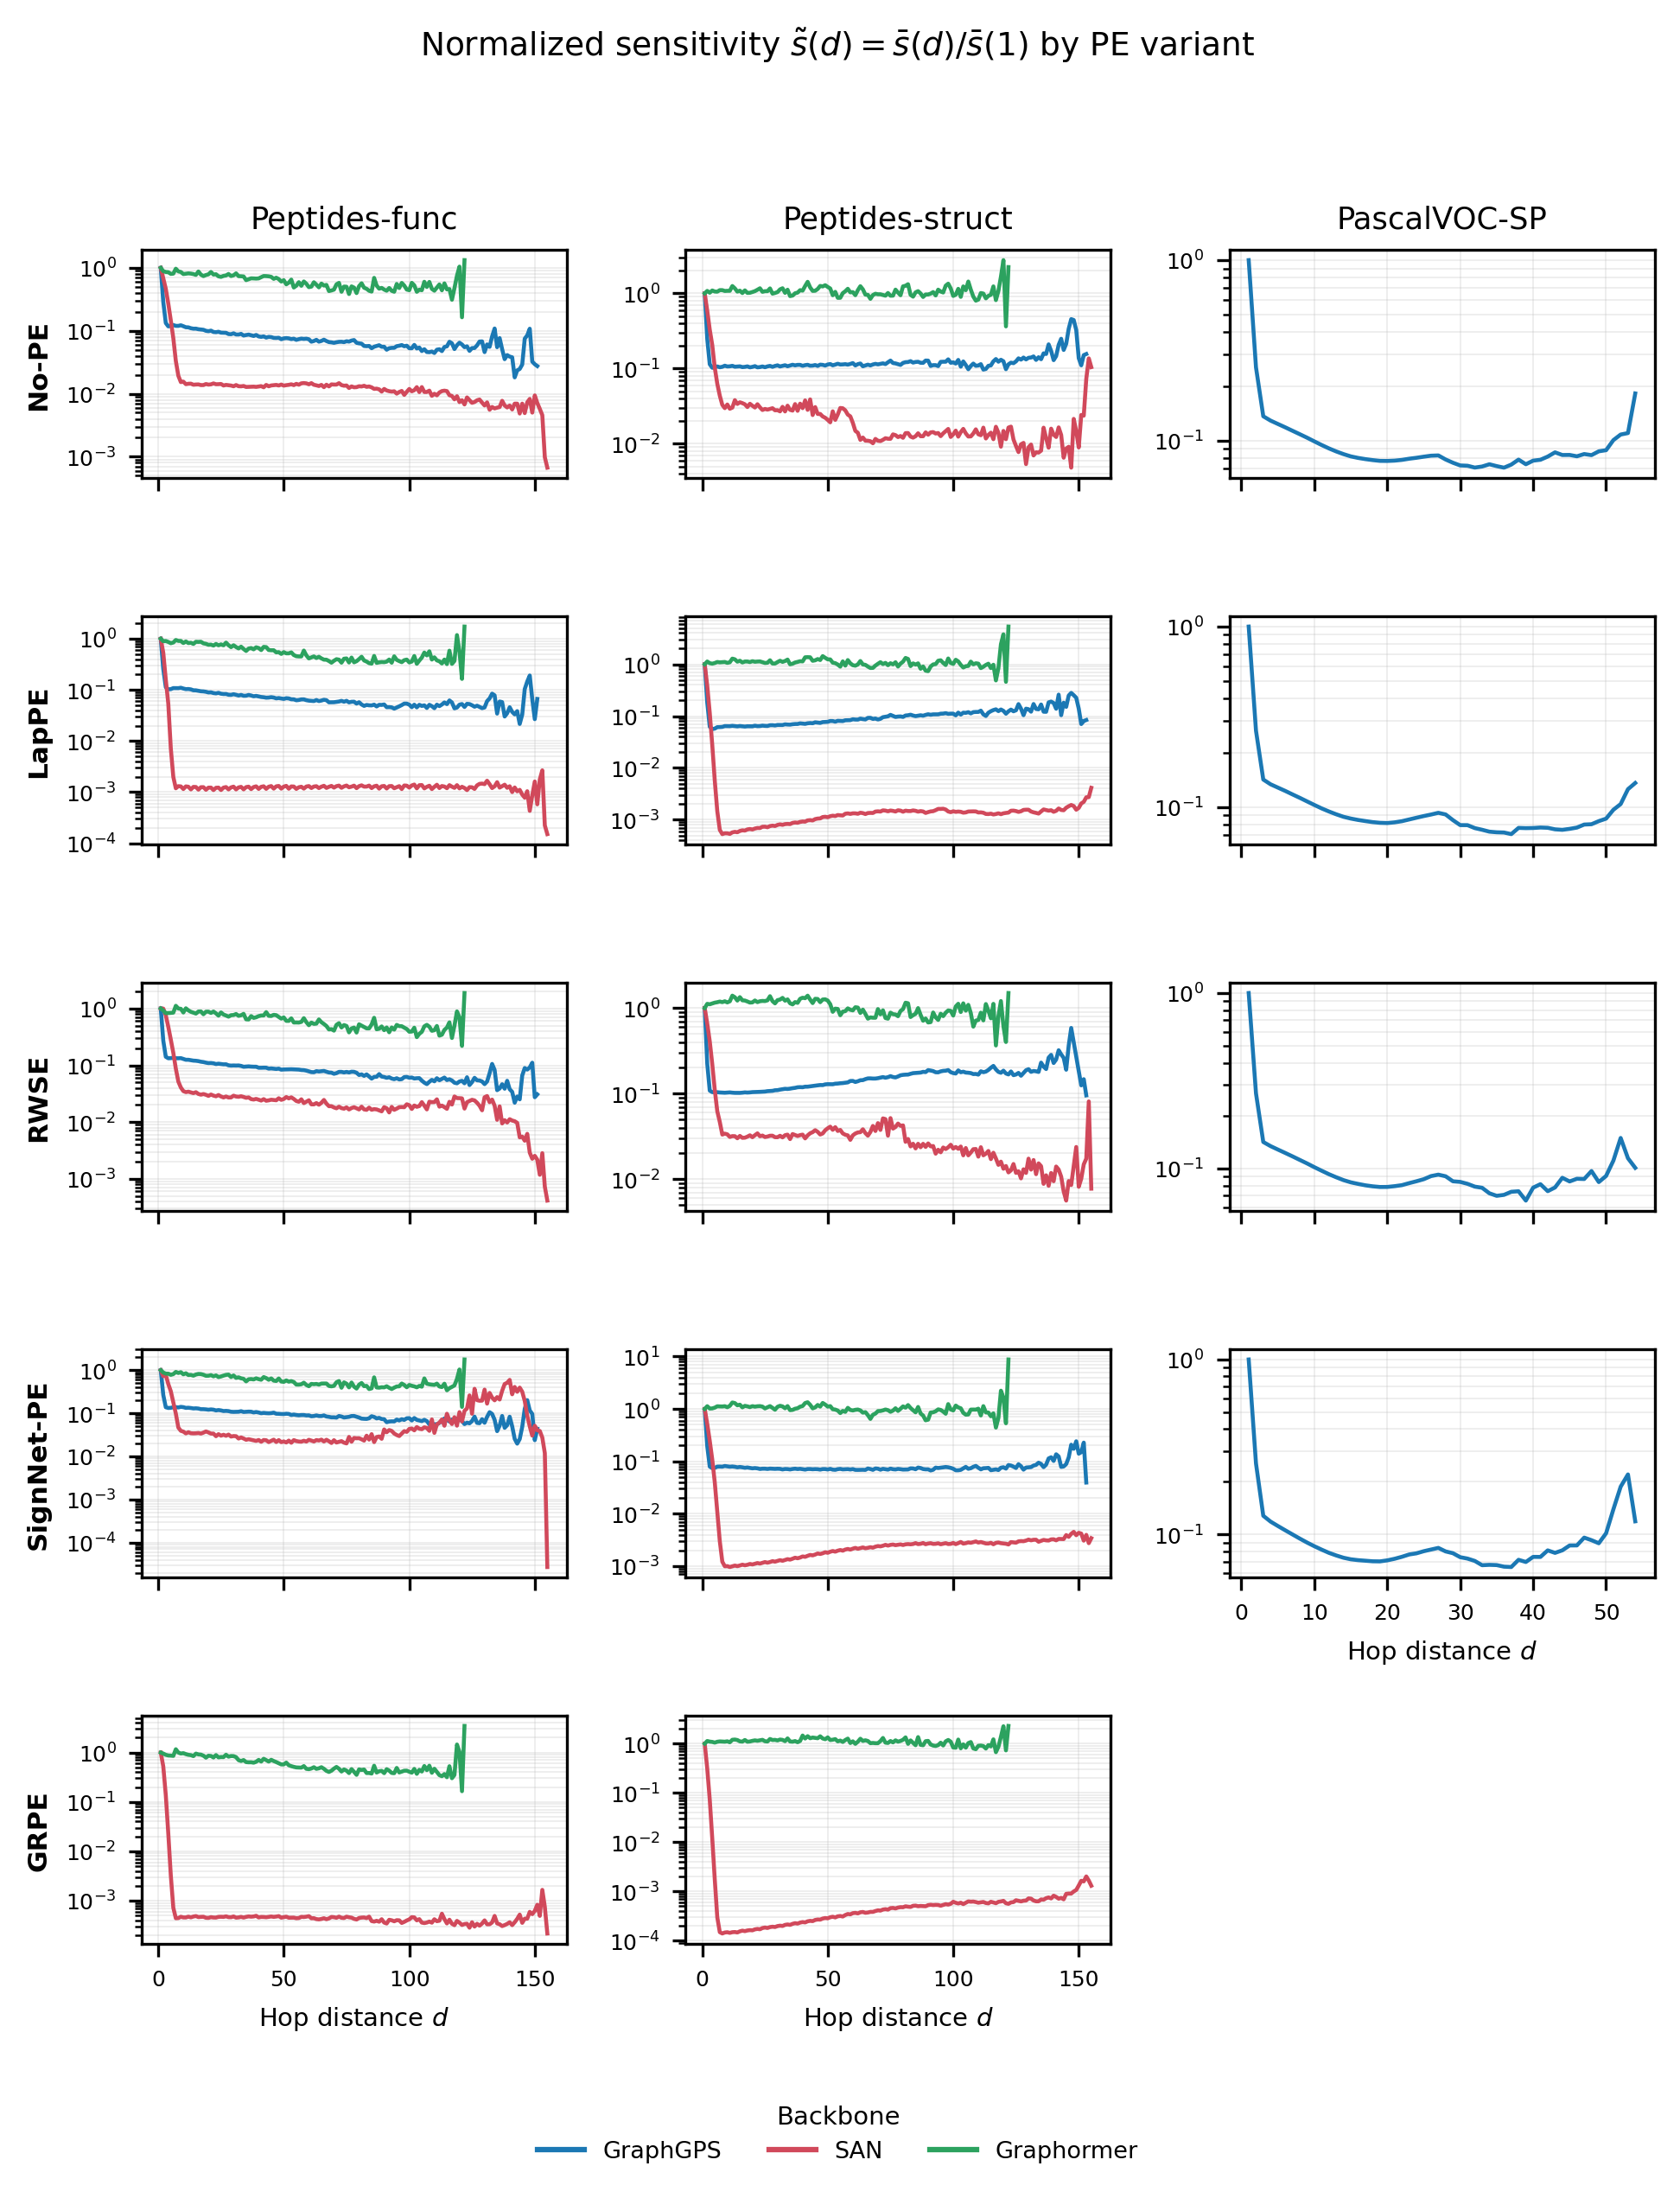
\includegraphics[width=0.95\textwidth]{figures/sensitivity_norm_combined.png}
\caption{Normalized curves $\tilde s(d)=\bar s(d)/\bar s(1)$, one line per (backbone, PE), log-$y$: a gain difference is a vertical shift, decay shape is slope. Left to right: Peptides-func, Peptides-struct, PascalVOC-SP. Compare SAN's (red) curves between the two Peptides panels: LapPE/GRPE collapse toward the bottom in both, but SignNet-PE collapses with them only on Peptides-struct -- on Peptides-func it instead sits with RWSE near the top. That within-SAN inconsistency, not a clean two-group split, is what \S5.1 discusses.}
\label{fig:curves}
\end{figure*}

\subsection{Sensitivity--Performance Correlation and Cross-Backbone Agreement}
Table~\ref{tab:critb} gives the Spearman correlation between $\rho_{\text{rel}}$ and task metric, MAE flipped so a \emph{negative} $r$ is the "more local $\Rightarrow$ better task" case (the table's caption has the full sign convention), per backbone (descriptive, $n\le5$) and pooled per dataset (confirmatory). $p$-values are exact permutation tests, not the asymptotic approximation, which is invalid at this $n$ and previously reported impossible values ($p{=}0$, $p{=}1.4\times10^{-23}$) -- see the caption for which rows still use the asymptotic fallback.

% Auto-generated by scripts/make_paper_tables.py -- do not hand-edit.
% Per-backbone rows are DESCRIPTIVE (n<=5 PEs, underpowered on their own,
% analysis-plan.md Amendment 3); 'ALL (pooled)' pools every (backbone, PE)
% arm for that dataset into one Spearman test and is the CONFIRMATORY read.
\begin{table}[h]
\centering\footnotesize
\setlength{\tabcolsep}{4pt}
\begin{tabular}{llrrr}
\toprule
\textbf{Dataset} & \textbf{Backbone} & \textbf{$n$} & \textbf{Spearman $r$} & \textbf{$p$} \\
\midrule
Peptides-func & GraphGPS & 4 & -1.00 & 0.0833 \\
Peptides-func & Graphormer & 5 & -0.60 & 0.35 \\
Peptides-func & SAN & 5 & -0.90 & 0.0833 \\
Peptides-func & ALL (pooled) & 14 & \textbf{0.41} & 0.149$^{\dagger}$ \\
\addlinespace
Peptides-struct & GraphGPS & 4 & -0.80 & 0.333 \\
Peptides-struct & Graphormer & 5 & 1.00 & 0.0167 \\
Peptides-struct & SAN & 5 & -0.80 & 0.133 \\
Peptides-struct & ALL (pooled) & 14 & \textbf{0.53} & 0.0514$^{\dagger}$ \\
\addlinespace
PascalVOC-SP & GraphGPS & 4 & 0.20 & 0.917 \\
PascalVOC-SP & SAN & 5 & -- & undef. \\
PascalVOC-SP & ALL (pooled) & 9 & \textbf{0.84} & 0.00926 \\
\addlinespace
\bottomrule
\end{tabular}
\caption{Criterion (b): Spearman rank correlation between $\rho_{\text{rel}}$ and the task metric. MAE is sign-flipped so a higher task-metric value always means better task performance; $\rho_{\text{rel}}$ itself is not sign-flipped, so a \emph{negative} $r$ is the ``more local $\Rightarrow$ better task'' case, not a positive one. $p$ is an exact permutation $p$-value, enumerating all $n!$ rank permutations, except the two $n{=}14$ pooled rows marked $^{\dagger}$, which fall back to the asymptotic approximation since $n!$ is too large to enumerate there. SAN's PascalVOC-SP row is ``undef.'': $\rho_{\text{rel}}=0$ identically for every PE there, so the correlation itself is not defined, not merely untested. Sign and magnitude both differ by backbone.}
\label{tab:critb}
\end{table}


GraphGPS and SAN agree in sign on both Peptides sets (negative: $r{=}{-1.00}/{-}0.80$ and $-0.90/-0.80$), though none individually clears $p<0.05$ at $n{\le}5$ -- Amendment 3's power warning, not a contradiction of the pooled row. Graphormer's own correlation ($r{=}1.00$ struct, $-0.60$ func) is not treated as informative: it is built from PEs whose entire $\rho_{\text{rel}}$ span is smaller than Graphormer's own measurement noise (\S5.1), so no permutation $p$-value on the ranks can rescue what the ranks themselves cannot resolve. The pooled correlations are significant on PascalVOC-SP ($r{=}0.84$) and marginal on Peptides-struct ($r{=}0.53$), and neither should be read as a clean confirmation. VOC's is a two-cluster artifact, not a within-backbone relationship: SAN's five points all sit at $\rho_{\text{rel}}{=}0$, degenerate per \S5.1, with F1 uniformly below every GraphGPS point, so the correlation just says SAN is worse than GraphGPS on both axes. Struct's 14 pooled points, in turn, include Graphormer's three unreliable ones.

Do backbones at least agree on the sensitivity \emph{ranking}? Kendall's $W$, with an exact permutation $p$-value enumerating all $(n!)^m$ null rank-matrices rather than the asymptotic chi-square, gives $W{=}0.82$, $p{=}0.033$ on Peptides-struct ($n{=}4$ PEs, $m{=}3$ backbones) -- \textbf{significant}, correcting an earlier asymptotic estimate of $p{=}0.060$ we had read as marginal. GraphGPS, SAN and Graphormer all rank SignNet-PE/LapPE more local than RWSE/No-PE there once GRPE is dropped. On Peptides-func, $W{=}0.56$, $p{=}0.207$. \textbf{This significance is fragile to exactly the backbone we trust least}: dropping Graphormer gives $W{=}0.800$ (barely smaller) but $p{=}0.208$ (no longer significant) -- a 2-rater exact test has far less power at this $n$, so Graphormer's inclusion is what crosses $\alpha{=}0.05$, and it is the rater with 25$\times$ less probe data (\S4). PascalVOC-SP is untestable: SAN's ranking there is an all-way tie.

No best-PE-per-cell transfers across backbones or datasets either: LapPE is GraphGPS's best PE on Peptides-struct (MAE 0.251) yet SAN's second-worst there (MAE 0.296, ahead of only No-PE) on the identical graphs; GraphGPS and SAN agree no PE helps sensitivity on PascalVOC-SP but disagree completely on whether PEs help the task (every PE hurts GraphGPS's F1, every PE helps SAN's). PE effects on sensitivity and on task performance are both backbone-conditional -- exactly what a single-backbone study cannot rule out. Table~\ref{tab:headline} distills this into the one artifact meant to carry the claim on its own: rank-agreement is high where it matters (Peptides-struct) and the correlation sign still splits 2-1 against it.

% Auto-generated by scripts/make_paper_tables.py -- do not hand-edit.
% W is a DATASET-level number (repeated per backbone row on purpose --
% it is a property of how the backbones agree, not of one backbone);
% correlation sign is a BACKBONE-level number (from criterion_b_*.csv).
\begin{table}[h]
\centering\footnotesize
\setlength{\tabcolsep}{4pt}
\begin{tabular}{llcc}
\toprule
\textbf{Dataset} & \textbf{Backbone} & \textbf{Rank-agr.\ ($W$)} & \textbf{Corr.\ sign} \\
\midrule
Peptides-func & GraphGPS & 0.56 & $-$ (-1.00) \\
Peptides-func & Graphormer & 0.56 & $-$ (-0.60) \\
Peptides-func & SAN & 0.56 & $-$ (-0.90) \\
\addlinespace[1pt]
Peptides-struct & GraphGPS & 0.82 & $-$ (-0.80) \\
Peptides-struct & Graphormer & 0.82 & $+$ (1.00) \\
Peptides-struct & SAN & 0.82 & $-$ (-0.80) \\
\addlinespace[1pt]
PascalVOC-SP & GraphGPS & n/a & $+$ (0.20) \\
PascalVOC-SP & Graphormer & n/a & n/a \\
PascalVOC-SP & SAN & n/a & n/a (degenerate) \\
\addlinespace[1pt]
\bottomrule
\end{tabular}
\caption{Headline claim, distilled. \textbf{Rank-agr.\ ($W$)}: Kendall's coefficient of concordance between backbones' $\rho_{\text{rel}}$ rankings of PEs on that dataset (\S5.2) -- a property of the dataset, identical across its backbone rows here. \textbf{Corr.\ sign}: sign of that backbone's own Spearman $r$ between $\rho_{\text{rel}}$ and task metric (Table~\ref{tab:critb}) -- a property of the backbone. High $W$ with disagreeing signs (Peptides-struct) is the paper's central finding: backbones agree which PE is more local, not on what that locality means for the task.}
\label{tab:headline}
\end{table}


\begin{figure*}[t]
\centering
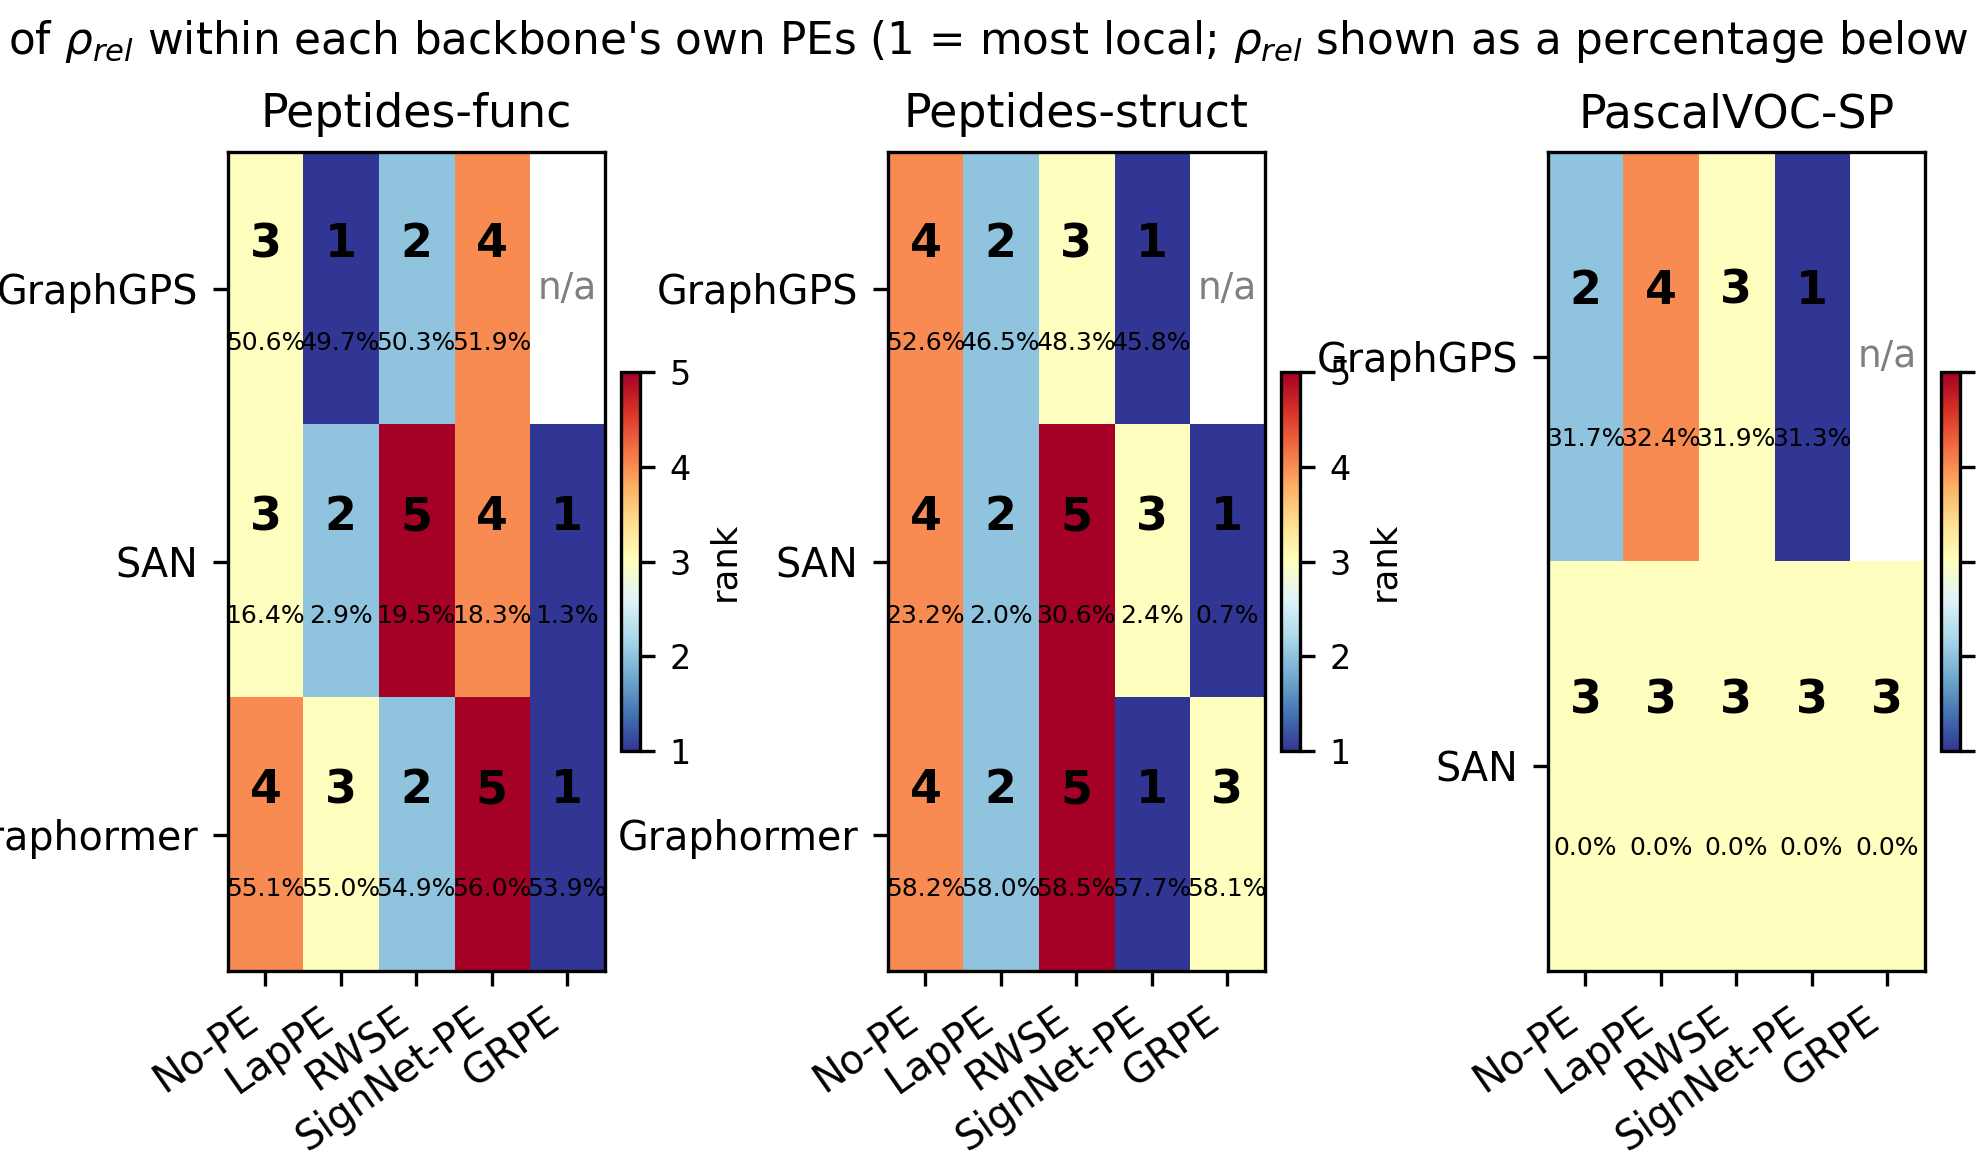
\includegraphics[width=0.95\textwidth]{figures/ranking_heatmap_combined.png}
\caption{Rank of $\rho_{\text{rel}}$ within each backbone's own PEs (bold, 1=most local; $\rho_{\text{rel}}$ shown as a percentage below it; blank=never ran). Peptides-func, Peptides-struct, PascalVOC-SP, left to right.}
\label{fig:ranking}
\end{figure*}

\subsection{Paired Bootstrap on Peptides-func}
Table~\ref{tab:results}'s CIs are marginal (arm vs.\ arm separately); pairing each PE against its own No-PE arm \emph{by graph identity} and bootstrapping the difference cancels shared between-graph variance -- flagged as the most promising unresolved analysis in our prior work (\texttt{docs/findings\_gps.txt} \S9). It sharpens GraphGPS's Peptides-func picture, where the marginal comparison (\S5.1) left only one razor-thin star: LapPE shows a significant negative paired effect ($\Delta\rho_{\text{rel}}{=}{-}0.0072$, CI $[-0.0107,-0.0037]$) and SignNet-PE a significant positive one ($+0.0146$, CI $[0.0102,0.0189]$) -- small but real by this tighter method, and opposite in sign despite both improving AP. The same method must \emph{not} be over-read on PascalVOC-SP: it resamples graphs but not seeds, and GraphGPS's VOC arm is exactly where prior analysis found between-seed variance dominant, so its "significant" LapPE/RWSE paired effects there ($+0.0077$, $+0.0044$) likely repeat that same false-positive rather than confirm a new one (full numbers in \texttt{results\_all/paired\_bootstrap.csv}).

\section{Discussion}
GraphGPS's Peptides-struct result -- task-improving PEs pull sensitivity mass toward the near half, not the far half -- reappears in direction on SAN despite SAN's near-total collapse under three of five PEs, suggesting it is not specific to GraphGPS's GatedGCN+Transformer hybrid. Whether it reverses under Graphormer is the one question here we cannot answer: its $\rho_{\text{rel}}$ range (0.577--0.585, span 0.0074) is narrow enough to fit either "PEs genuinely barely differ" or pure sampling noise, since its own CI width ($\sim$0.036) and seed sd (up to 0.024) both dwarf that span (\S4/\S5.1). The two explanations predict the identical symptom and nothing here distinguishes them; re-probing at 256 graphs (no retraining needed) would. Until then, Graphormer's contribution to the headline is \emph{not measured precisely enough to say}, not evidence PEs work oppositely on attention-only backbones.

SAN's LapPE/GRPE collapse and RWSE elevation are consistent across both Peptides datasets (built from identical graphs), which has no counterpart in GraphGPS and is not predicted by the equi-expressivity results we build on (Black et al., 2024) -- expressivity says nothing about which mechanism a gradient prefers. SignNet-PE is not consistent: it groups with RWSE on Peptides-func and with the collapsed pair on Peptides-struct. We do not have a mechanistic explanation for this split: all four PEs route through the identical LPE dispatch slot in SAN's implementation (\S5.1), differing only in an internal encoder variant, so ``how the PE enters the model'' does not distinguish them. Two real, disclosed confounds are at least partial alternative explanations rather than a mechanism (Limitations): on Peptides-func the collapsed-vs-elevated split is perfectly confounded with parameter count (LapPE/GRPE $\approx$928K vs.\ No-PE/RWSE/SignNet-PE $\approx$791--793K), but that confound does \emph{not} hold on Peptides-struct, where LapPE and No-PE are both $\approx$928K yet $\rho_{\text{rel}}$ is 0.020 vs.\ 0.232 -- so parameter count is a candidate explanation for func alone, not a rebuttal of the struct split. GraphGPS's GRPE cell never training still removes the one three-way native-vs-adapted GRPE comparison we planned; the two-way comparison available (Graphormer native vs.\ SAN adapted) is at least consistent with GRPE not stabilizing across backbones, though two backbones cannot generalize.

\section{Limitations}
\begin{itemize}[leftmargin=1.1em, itemsep=0pt, topsep=1pt]
\item \textbf{Graphormer's probe used 10 test graphs/seed, not 256} -- the single most consequential item here; full numbers and which claims it downgrades are in \S4/\S5.1/\S6, not repeated here.
\item \textbf{GraphGPS+GRPE never trained} (attention-bias hook designed, not wired); GraphGPS has 4 PE arms, not 5, throughout.
\item \textbf{Graphormer's PascalVOC-SP arm never trained} in our compute budget (a resource statement, not an architectural one -- \S4); no 3-backbone comparison exists there.
\item \textbf{SAN's PascalVOC-SP arm is degenerate, not null} (\S5.1): $\rho_{\text{rel}}{=}0$ by construction, and the VOC pooled correlation in \S5.2 is partly built from these invalid numbers.
\item \textbf{SignNet-PE is off its parameter budget} on GraphGPS (576,138 vs.\ $\approx$503--507K, +14\%) and on PascalVOC-SP, and trains at a different batch/accumulation split -- disclosed here because it carries a starred Peptides-func result and a third of the Peptides-struct trio, not only null ones.
\item \textbf{SAN's param count perfectly predicts its Peptides-func collapse split} but not Peptides-struct's (\S6) -- a partial, dataset-specific alternative to the mechanism-free reading, not a rebuttal of it.
\item \textbf{SAN's $T{=}128$ probe budget saturates} (enumerates rather than samples) for any graph $\le128$ nodes, roughly half its pool.
\item Training budgets follow each backbone's own reference recipe (unequalized epochs), a difference along the axis \S5.2 compares.
\item \textbf{The Jacobian uses each backbone's full hidden width}, PE channels included but constant across a backbone's own PEs (\S3.2) -- not the content-only exclusion an earlier draft described.
\item \textbf{The paired bootstrap (\S5.3) resamples graphs, not seeds}, so it can repeat a seed-variance false positive where that dominates (GraphGPS VOC); only its Peptides-func result is read as confirmed.
\item The sensitivity metric is a first-order, input-gradient measure -- a lower bound on long-range capacity, not a full characterization.
\end{itemize}

\section{Conclusion}
This report extended a single-backbone, single-dataset PE-sensitivity study into a partial 3-backbone $\times$ 5-PE $\times$ 3-dataset grid (37/45 cells, all 3 seeds, though not all with the same probe budget), testing whether a PE ranking from one backbone/dataset generalizes. Between the two backbones we can actually trust equally, it does not transfer cleanly either: GraphGPS and SAN agree which PE is more local on Peptides-struct ($W{=}0.82$, exact $p{=}0.033$, GraphGPS+SAN alone) and agree in sign that more-local PEs help the task there, but disagree completely on PascalVOC-SP (every PE hurts GraphGPS, every PE helps SAN), and within SAN itself, SignNet-PE's inconsistency across two datasets built from the same graphs rules out ``how the PE enters the model'' as a sufficient explanation for its own LapPE/GRPE-vs-RWSE split (\S6) -- a real finding, not an artifact of the mechanistic story we originally proposed for it, which turned out to be false (\S5.1). Graphormer cannot yet be added to either conclusion: its probe used 25$\times$ fewer test graphs than the other two backbones, an omission this revision corrects by disclosing rather than by re-running, and every Graphormer-dependent number in \S5--\S6 is marked accordingly. The pooled sensitivity--performance correlation is significant on PascalVOC-SP but is a two-cluster artifact built partly from SAN's invalid degenerate sensitivity numbers, and the Peptides-struct pooled correlation includes Graphormer's unreliable points among its 14; neither should be read as backbone-general evidence. The repository (\texttt{scripts/\allowbreak collect\_cross\_backbone\_results.py}, \texttt{aggregate\_results.py}, \texttt{make\_paper\_tables.py}, \texttt{paired\_bootstrap.py}, \texttt{make\_ranking\_figures.py}) reproduces every number here from the three backbone branches; re-probing Graphormer at 256 graphs, filling GraphGPS+GRPE, and training Graphormer's PascalVOC-SP arm are the concrete next steps before these cross-backbone claims can be stated without the caveats in \S7.

\begin{thebibliography}{99}
\small
\bibitem[Alon and Yahav, 2021]{alon2021} U. Alon and E. Yahav. On the bottleneck of graph neural networks and its practical implications. \emph{ICLR}, 2021.
\bibitem[Bechler-Speicher et al., 2025]{bs2025} M. Bechler-Speicher et al. Position: Graph Learning Will Lose Relevance Due To Poor Benchmarks. \emph{arXiv:2502.14546}, 2025.
\bibitem[Black et al., 2024]{black2024} M. Black et al. Comparing graph transformers via positional encodings. \emph{ICML}, 2024. arXiv:2402.14202.
\bibitem[Di Giovanni et al., 2023]{digiovanni2023} F. Di Giovanni et al. On over-squashing in message passing neural networks. \emph{ICML}, 2023.
\bibitem[Dwivedi and Bresson, 2020]{dwivedi2020} V. P. Dwivedi and X. Bresson. A generalization of transformer networks to graphs. \emph{arXiv:2012.09699}, 2020.
\bibitem[Dwivedi et al., 2022]{dwivedi2022} V. P. Dwivedi et al. Long range graph benchmark. \emph{NeurIPS Datasets \& Benchmarks}, 2022. arXiv:2206.08164.
\bibitem[Errica et al., 2020]{errica2020} F. Errica, M. Podda, D. Bacciu, A. Micheli. A fair comparison of graph neural networks for graph classification. \emph{ICLR}, 2020.
\bibitem[Kreuzer et al., 2021]{kreuzer2021} D. Kreuzer, D. Beaini, W. L. Hamilton, V. L\'etourneau, P. Tossou. Rethinking graph transformers with spectral attention. \emph{NeurIPS}, 2021. arXiv:2106.03893.
\bibitem[Lim et al., 2023]{lim2023} D. Lim et al. Sign and basis invariant networks for spectral graph representation learning. \emph{ICLR}, 2023. arXiv:2202.13013.
\bibitem[Park et al., 2022]{park2022} W. Park, W.-G. Chang, D. Lee, J. Kim, et al. GRPE: Relative positional encoding for graph transformer. \emph{ICLR MLDD Workshop}, 2022. arXiv:2201.12787.
\bibitem[Rampasek et al., 2022]{rampasek2022} L. Rampasek et al. Recipe for a general, powerful, scalable graph transformer. \emph{NeurIPS}, 2022.
\bibitem[Ying et al., 2021]{ying2021} C. Ying et al. Do transformers really perform bad for graph representation? \emph{NeurIPS}, 2021. arXiv:2106.05234.
\end{thebibliography}

\end{document}
